\documentclass{classes/exam} 
\usepackage{chemfig}
\usepackage{tikz}
\usepackage{physics}
\usepackage{circuitikz}
\usepackage{graphicx}
\graphicspath{ {./images/} }
\usepackage[version=4]{mhchem}
\usepackage{tkz-euclide}
\definecolor{myyellow}{RGB}{254,241,24}
\definecolor{myorange}{RGB}{234,125,1}
\usepackage{tkz-euclide}
\usetkzobj{all}
\tikzstyle arrowstyle=[scale=1]
\tikzstyle directed=[postaction={decorate,decoration={markings,
		mark=at position .65 with {\arrow[arrowstyle]{stealth}}}}]
\tikzstyle direct=[postaction={decorate,decoration={markings,
		mark=at position .65 with {\arrow[arrowstyle]{stealth reversed}}}}]
\usetikzlibrary{shadings,shapes.geometric,calc, patterns, angles, quotes, arrows.meta, shapes, decorations.pathmorphing, decorations.shapes, decorations.text,calc,angles,quotes,decorations.markings}
\tikzset{>=latex}
\usepackage{chemfig}
\usepackage{multirow}
\usetikzlibrary{quotes,arrows.meta}
%%%%%%%%%%%%%%%%%%%%%%%%%%%%%%%%%Declarations%%%%%%%%%%%%%%%%%%%%%%%%%%%%%%%%%%%%

\begin{document}
	\maketitle
	\borderline{ប្រធាន}
	\begin{enumerate}[I]
		\item {\color{magenta}\ks (៥ ពិន្ទុ)} បញ្ជាក់លក្ខណៈខុសគ្នារវាងទំហំវ៉ិចទ័រ និងទំហំស្កាលែ រួចលើកឧទាហរណ៍អំពីទំហំនីមួយៗ។
		\item {\color{magenta}\ks (១០ ពិន្ទុ)} អ្នកចង់រកកំពស់ដើមឈើតែមិនអាចវាស់ដោយផ្ទាល់បានទេ។ អ្នកឈរចម្ងាយ $50.0m$ ពីដើមឈើហើយកំណត់ថា បន្ទាត់នៃការមើលឃើញពីដីទៅដល់កំពូលនៃដើមឈើបង្កើតបានមុំ $30.0^\circ$ ជាមួយនឹងដី។ \\គណនាប្រវែង $\ell$ និងកម្ពស់ដើមឈើ $h$។ គេឲ្យៈ $\cos 30.0^\circ =0.866$,~ $\sin 30.0^\circ =0.5$  និង $\tan 30.0^\circ =0.577$
		\begin{figure}[H]
			\centering
			\begin{tikzpicture}[scale=.8, draw=magenta, fill=magenta]
			\begin{scope}
			\coordinate (O) at (0,0);
			\coordinate (A) at (-10,-2);
			\coordinate (B) at (0,-2);
			\coordinate (C) at (0,2);
			\node at (O) {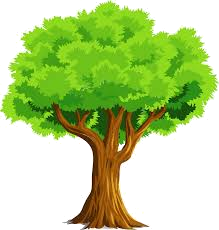
\includegraphics[scale=.4]{tree}};
			\node at (-10.2,-1.1) {
\includegraphics[scale=.25]{girl}};
			\draw[line width=1.5pt] (A) -- (B);
			\draw[line width=1.5pt] (B) -- (C);
			\draw[line width=1.5pt] (C) -- (A);
			\pic [draw, "$30.0^\circ$", angle eccentricity=1.5, angle radius=2cm] {angle= B--A--C};
			\draw[->, line width=1.5pt] (.5,-.5) -- (.5,2);
			\draw[->, line width=1.5pt] (.5,-1) -- (.5,-2);
			\node at (.5, -.8) {$h$};
			\draw[->, line width=1.5pt] (-5.8,-2.5) -- (-10,-2.5);
			\draw[->, line width=1.5pt] (-4.2,-2.5) -- (0,-2.5);
			\node at (-5, -2.5) {$50.0m$};
			\draw[->, line width=1.5pt] (-5,.5) -- (-10,-1.5);
			\node[rotate=30] at (-4.7,.8) {$\ell$};
			\draw[->, line width=1.5pt] (-4.2,.8) -- (0,2.5);
			\end{scope}
			\end{tikzpicture}
%			\caption{\ak \color{magenta}លំហាត់ទី២}
		\end{figure}
		\item {\color{magenta}\ks (១០ ពិន្ទុ)} រកបម្លាស់ទីតាមអ័ក្សអាប់ស៊ីស និងអ័ក្សអរដោនេនៃបម្លាស់ទី $100.0m$ របស់កំពូលវីរបុរសម្នាក់បានហោះចេញពីកំពូលនៃដំបូលអាគារមួយដូចបានបង្ហាញក្នុងរូប។ គេឲ្យៈ $\cos 30.0^\circ =0.866$ និង $\sin 30.0^\circ =0.5$
		\begin{figure}[H]
			\centering
			\begin{tikzpicture}[scale=1, draw=magenta, fill=magenta]
			\coordinate (O) at (-.7,1.6);
			\coordinate[label=right:$x$] (X) at (2,1.6);
			\coordinate[label=left:$y$] (Y) at (-.7,2.2);
			\coordinate (M) at (1.2,-.2);
			\coordinate (B) at (-2,0);
			\node at (1,0) {
\includegraphics[scale=.25]{super-hero}};
			\node at (B) {
\includegraphics[scale=.7]{building}};
			\draw[->] (-.7,0) -- (Y);
			\node[rotate=-45] at (-.2,.5) {$100.0m$};
			\draw[->] (O) -- (X);
			\pic [draw, "$30.0^\circ$", angle eccentricity=1.5, angle radius=1cm] {angle= M--O--X};
			\draw[->, draw=cyan, line width=2pt] (O) -- (M);
			\end{tikzpicture}
%			\caption{\ak \color{magenta}លំហាត់ទី៣}
		\end{figure}
		\item {\color{magenta}\ks (១០ ពិន្ទុ)} រថភ្លើងពីរកំពុងផ្លាស់ទីមកជិតគ្នាទៅវិញទៅមកលើគន្លងស្របគ្នា ដែលរថភ្លើងនីមួយៗផ្លាស់ទីដោយល្បឿន $155km/h$ ធៀបនឹងដី។ ប្រសិនបើដំបូងរថភ្លើងទាំងពីរនេះស្ថិតនៅចម្ងាយពីគ្នាប្រវែង $8.5km$។\\ តើរយៈពេលប៉ុន្មាននាទីទើបរថភ្លើងទាំងពីរជួបគ្នា?
		\begin{figure}[H]
			\centering
			\begin{tikzpicture}[draw=magenta, fill=magenta]
			\begin{scope}
			\draw[->, line width=3pt] (-1.5,.5) --(-.5,.5);
			\draw[->, line width=3pt] (1.5,.5) --(.5,.5);
			\draw[->] (.8,2) --(1.5,2);
			\node at (0,2) {$8.5km$};
			\draw[->] (-.8,2) --(-1.5,2);
			\coordinate[label=above:${\upsilon=155km/h}$] (v1) at (-1,1);
			\coordinate[label=above:${\upsilon=155km/h}$] (v2) at (1.8,1);
			\node at (0,0) {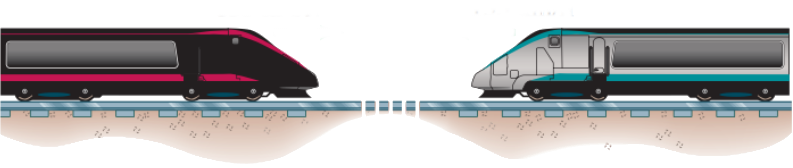
\includegraphics[scale=.4]{train1}};
			\end{scope}
			\end{tikzpicture}
%			\caption{\ak \color{magenta}លំហាត់ទី៤}
		\end{figure}
		\item {\color{magenta}\ks (១៥ ពិន្ទុ)} វ៉ិចទ័រនៃកម្លាំងពីរ $\overrightarrow{F}_{1}$ និង $\overrightarrow{F}_{2}$ មានអំពើលើវត្ថុមួយដែល $F_{1}=20.0N$ និង $F_{2}=15.0N$។\\ ចូរគណនាកម្លាំងផ្គួបដែលមានលើវត្ថុនេះក្នុងករណី \emph{\color{magenta}\kml ក,ខ} និង \emph{\color{magenta}\kml គ}។ គេឲ្យៈ $\cos 60.0^\circ =0.5$ និង $\cos 120.0^\circ =-0.5$
		\begin{enumerate}[k,3]
			\item \begin{tikzpicture}[draw=magenta, fill=magenta]
			\begin{scope}
			\coordinate (O) at (0,0);
			\coordinate[label=right:$\overrightarrow{F}_{1}$] (F1) at (2,0);
			\coordinate[label=above:$\overrightarrow{F}_{2}$] (F2) at (0,2);
			\draw [->, line width =2pt] (O) -- (F1);
			\draw [->, line width =2pt] (O) -- (F2); 
			\shade [ball color=cyan!20!white] (O) circle [radius=10pt];
			\node at (O) {$m$};
			\pic [draw, "$90.0^\circ$", angle eccentricity=1.7, angle radius=.7cm] {angle= F1--O--F2};
			\end{scope}
			\end{tikzpicture}
			\item \begin{tikzpicture}[draw=magenta, fill=magenta]
			\begin{scope}
			\coordinate (O) at (0,0);
			\coordinate[label=right:$\overrightarrow{F}_{1}$] (F1) at (2,0);
			\coordinate[label=above:$\overrightarrow{F}_{2}$] (F2) at (2,2);
			\draw [->, line width =2pt] (O) -- (F1);
			\draw [->, line width =2pt] (O) -- (F2); 
			\shade [ball color=cyan!20!white] (O) circle [radius=10pt];
			\node at (O) {$m$};
			\pic [draw, "$60.0^\circ$", angle eccentricity=1.5, angle radius=1cm] {angle= F1--O--F2};
			\end{scope}
			\end{tikzpicture}
			\item \begin{tikzpicture}[draw=magenta, fill=magenta]
			\begin{scope}
			\coordinate (O) at (0,0);
			\coordinate[label=right:$\overrightarrow{F}_{1}$] (F1) at (2,0);
			\coordinate[label=above:$\overrightarrow{F}_{2}$] (F2) at (-2,2);
			\draw [->, line width =2pt] (O) -- (F1);
			\draw [->, line width =2pt] (O) -- (F2); 
			\shade [ball color=cyan!20!white] (O) circle [radius=10pt];
			\node at (O) {$m$};
			\pic [draw, "$120.0^\circ$", angle eccentricity=1.5, angle radius=.7cm] {angle= F1--O--F2};
			\end{scope}
			\end{tikzpicture}
		\end{enumerate}
	\end{enumerate}
\newpage
\borderline{អត្រាកំណែ}
\begin{enumerate}[I]
	\item {\color{magenta}\ks (៥ ពិន្ទុ)}
		\begin{itemize}
			\item ទំហំវ៉ិចទ័រជាទំហំដែលសម្តែងជាតម្លៃពីជគណិតដោយអាស្រ័យនឹងទិស និងទិសដៅ។
			\item ទំហំស្កាលែជាទំហំដែលសម្តែងជាតម្លៃពីជគណិតដោយមិនអាស្រ័យនឹងទិស និងទិសដៅ។
		\end{itemize}
		\begin{itemize}
			\item ទំហំវ៉ិចទ័រ៖ កម្លាំង ល្បឿន សំទុះ ទម្ងន់ បម្លាស់ទី។ល។
			\item ទំហំស្កាលែ៖ សម្ពាធ កម្តៅ រយៈពេល ចម្ងាយចរ មាឌ។ល។
		\end{itemize}
	\item {\color{magenta}\ks (១០ ពិន្ទុ)} គណនាប្រវែង $\ell$ និងកម្ពស់ដើមឈើ $h$។
	\begin{figure}[H]
		\centering
		\begin{tikzpicture}[scale=.8, draw=magenta, fill=magenta]
		\begin{scope}
		\coordinate (O) at (0,0);
		\coordinate (A) at (-10,-2);
		\coordinate (B) at (0,-2);
		\coordinate (C) at (0,2);
		\node at (O) {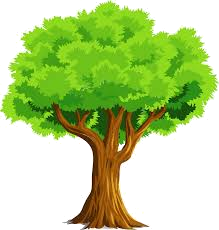
\includegraphics[scale=.4]{tree}};
		\node at (-10.2,-1.1) {
\includegraphics[scale=.25]{girl}};
		\draw[line width=1.5pt] (A) -- (B);
		\draw[line width=1.5pt] (B) -- (C);
		\draw[line width=1.5pt] (C) -- (A);
		\pic [draw, "$30.0^\circ$", angle eccentricity=1.5, angle radius=2cm] {angle= B--A--C};
		\draw[->, line width=1.5pt] (.5,-.5) -- (.5,2);
		\draw[->, line width=1.5pt] (.5,-1) -- (.5,-2);
		\node at (.5, -.8) {$h$};
		\draw[->, line width=1.5pt] (-5.8,-2.5) -- (-10,-2.5);
		\draw[->, line width=1.5pt] (-4.2,-2.5) -- (0,-2.5);
		\node at (-5, -2.5) {$50.0m$};
		\draw[->, line width=1.5pt] (-5,.5) -- (-10,-1.5);
		\node[rotate=35] at (-4.7,.8) {$\ell$};
		\draw[->, line width=1.5pt] (-4.2,.8) -- (0,2.5);
		\end{scope}
		\end{tikzpicture}
	\end{figure}
	\begin{enumerate}[k]
		\item របៀបទី១
		\begin{flalign*}
			\text{តាម}\quad :& \quad \tan30.0^\circ=\frac{h}{50.0}\\
			\text{នាំឲ្យ}\quad :&\quad h=0.577\times50.0= 28.8675m\approx 29.0m\\
			\text{ដូចនេះ}\quad :&\quad h= 28.8675m\approx 29.0m
			\end{flalign*}
		\item របៀបទី២
		\begin{flalign*}
			\text{តាម}\quad :& \quad \cos30.0^\circ=\frac{50.0}{\ell}=\frac{50.0}{\cos30.0^\circ}\\
			\text{នាំឲ្យ}\quad :&\quad \ell=\frac{50.0}{0.866}= 57.7367m\\
			\text{គេបាន}\quad :&\quad \sin30.0^\circ=\frac{h}{\ell}\\
			\quad :&\quad h=\sin30.0^\circ\times\ell=0.5\times57.7367=28.86835m\approx29.0m\\
		 	\text{ដូចនេះ}\quad :&\quad \ell =57.7367m~\text{និង}~ h= 28.86835m\approx 29.0m
		\end{flalign*}
	\end{enumerate}
	\newpage
	\item {\color{magenta}\ks (១០ ពិន្ទុ)} រកបម្លាស់ទីតាមអ័ក្សអាប់ស៊ីស និងអ័ក្សអរដោនេ
	\begin{figure}[H]
		\centering
		\begin{tikzpicture}[scale=1.2, draw=magenta, fill=magenta]
		\coordinate (O) at (-.9,1.4);
		\coordinate[label=right:$x$] (X) at (2,1.4);
		\coordinate[label=left:$y$] (Y) at (-.9,2.5);
		\coordinate (M) at (1.2,-.2);
		\coordinate (B) at (-2,0);
		\coordinate [label=below right:{$d_{y}$}](dy) at (-.9,-.2);
		\coordinate [label=above:$d_{x}$](dx) at (1.2,1.4);
		\node at (1,0) {
\includegraphics[scale=.25]{super-hero}};
		\node at (B) {
\includegraphics[scale=.75]{building}};
		\draw[->] (-.9,-1) -- (Y);
		\draw[dashed] (1.2,-.2) -- (1.2,1.4);
		\draw[dashed] (1.2,-.2) -- (-.9,-.2);
		\node[rotate=-36] at (-.3,.5) {$100.0m$};
		\draw[->] (O) -- (X);
		\pic [draw, "$30.0^\circ$", angle eccentricity=1.5, angle radius=1cm] {angle= M--O--X};
		\draw[->, draw=cyan, line width=2pt] (O) -- (M);
		\end{tikzpicture}
	\end{figure}
	\begin{flalign*}
		\text{តាង}\quad :& \quad d_{x}\quad\text{ជាបម្លាស់ទីតាមអ័ក្សអាប់ស៊ីស}\\
		\quad :& \quad d_{y}\quad\text{ជាបម្លាស់ទីតាមអ័ក្សអរដោនេ}\\
		\text{តាម}\quad :&\quad \cos30.0^\circ=\frac{d_{x}}{100.0}\\
		\text{នាំឲ្យ}\quad :&\quad d_{x}=\cos30.0^\circ\times100.0=0.866\times100.0=86.6m\\
		\text{និង}\quad :&\quad \sin30.0^\circ=\frac{d_{y}}{100.0}\\
		\text{នាំឲ្យ}\quad :&\quad d_{y}=\sin30.0^\circ\times100.0=0.5\times100.0=50.0m\\
		\text{ដូចនេះ}\quad :&\quad d_{x}= 86.6m\quad \text{និង}\quad d_{y}= 50.0m 
	\end{flalign*}
	\item {\color{magenta}\ks (១០ ពិន្ទុ)} កំណត់រយៈពេលដែលរថភ្លើងទាំងពីរជួបគ្នា
	\begin{figure}[H]
		\centering
		\begin{tikzpicture}[draw=magenta, fill=magenta]
		\begin{scope}
		\draw[->, line width=3pt] (-1.5,.5) --(-.5,.5);
		\draw[->, line width=3pt] (1.5,.5) --(.5,.5);
		\draw[->] (.8,2) --(1.5,2);
		\node at (0,2) {$8.5km$};
		\draw[->] (-.8,2) --(-1.5,2);
		\coordinate[label=above:${\upsilon=155km/h}$] (v1) at (-1,1);
		\coordinate[label=above:${\upsilon=155km/h}$] (v2) at (1.8,1);
		\node at (0,0) {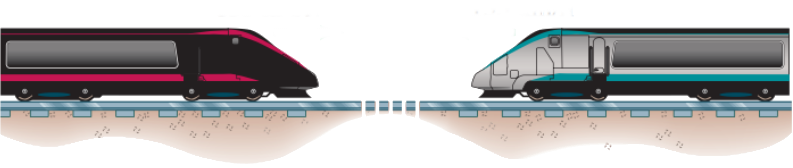
\includegraphics[scale=.4]{train1}};
		\end{scope}
		\end{tikzpicture}
	\end{figure}
	\begin{flalign*}
		\text{ដោយរថភ្លើងទាំងពីរមានផ្លាស់ទីដោយល្បឿនថេរ}\quad :&\quad \upsilon=155km/h\\
		\text{គេបានចម្ងាយដែលពេលវាជួបគ្នាគឺ}\quad :&\quad d=\frac{8.5km}{2}=4.25km\\
		\text{តាម}\quad :&\quad \upsilon_{av}=\frac{d}{\Delta t}\quad \text{នោះ}\quad \Delta t=\frac{d}{\upsilon_{av}}\\
		\quad :& \quad \Delta t=\frac{4.25km}{155km/h}=0.0274h\\
		\quad :& \quad \Delta t=0.0274h\left(\frac{60min}{1h}\right)=1.645min\\
		\text{ដូចនេះ}\quad :&\quad \Delta t= 1.645min\approx 1.6min\approx 90s
	\end{flalign*}
	\newpage
	\item {\color{magenta}\ks (១៥ ពិន្ទុ)} គណនាកម្លាំងផ្គួបដែលមានលើវត្ថុនេះក្នុងករណី
	\begin{enumerate}[k,2]
		\item \begin{tikzpicture}[scale=1, draw=magenta, fill=magenta]
					\begin{scope}
						\coordinate (O) at (0,0);
						\coordinate[label=right:$\overrightarrow{F}_{1}$] (F1) at (2,0);
						\coordinate[label=above:$\overrightarrow{F}_{2}$] (F2) at (0,2);
						\coordinate[label=above:$\overrightarrow{F}$] (F) at (2,2);
						\draw [->, line width =2pt] (O) -- (F1);
						\draw [->, line width =2pt] (O) -- (F2);
						\draw [->, line width =2pt] (O) -- (F);
						\shade [ball color=cyan!20!white] (O) circle [radius=10pt];
						\node at (O) {$m$};
						\pic [draw, "$90.0^\circ$", angle eccentricity=1.7, angle radius=.7cm] {angle= F1--O--F2};
						\draw[dashed] (F1)--(F);
						\draw[dashed] (F2)--(F);
					\end{scope}
				\end{tikzpicture}
			\item \begin{tikzpicture}[scale=1, draw=magenta, fill=magenta]
					\begin{scope}
						\coordinate (O) at (0,0);
						\coordinate[label=right:$\overrightarrow{F}_{1}$] (F1) at (2,0);
						\coordinate[label=above:$\overrightarrow{F}_{2}$] (F2) at (2,2);
						\coordinate[label=above:$\overrightarrow{F}$] (F) at (4,2);
						\draw [->, line width =2pt] (O) -- (F1);
						\draw [->, line width =2pt] (O) -- (F2); 
						\draw [->, line width =2pt] (O) -- (F);
						\shade [ball color=cyan!20!white] (O) circle [radius=10pt];
						\node at (O) {$m$};
						\pic [draw, "$60.0^\circ$", angle eccentricity=1.5, angle radius=1cm] {angle= F1--O--F2};
						\draw[dashed] (F1)--(F);
						\draw[dashed] (F2)--(F);
					\end{scope}
				\end{tikzpicture}
			\item \begin{tikzpicture}[scale=1, draw=magenta, fill=magenta]
					\begin{scope}
						\coordinate (O) at (0,0);
						\coordinate[label=right:$\overrightarrow{F}_{1}$] (F1) at (2,0);
						\coordinate[label=above:$\overrightarrow{F}_{2}$] (F2) at (-2,2);
						\coordinate[label=above:$\overrightarrow{F}$] (F) at (.5,2);
						\draw [->, line width =2pt] (O) -- (F1);
						\draw [->, line width =2pt] (O) -- (F2); 
						\draw [->, line width =2pt] (O) -- (F);
						\shade [ball color=cyan!20!white] (O) circle [radius=10pt];
						\node at (O) {$m$};
						\pic [draw, "$120.0^\circ$", angle eccentricity=1.5, angle radius=.7cm] {angle= F1--O--F2};
						\draw[dashed] (F1)--(F);
						\draw[dashed] (F2)--(F);
					\end{scope}
				\end{tikzpicture}
	\end{enumerate}
	\begin{enumerate}[k]
		\item ចំពោះរូប \emph{\color{magenta}\ks ក}
		\begin{flalign*}
			\text{តាមរូបគេបាន}\quad :&\quad \overrightarrow{F}=\overrightarrow{F}_{1}+\overrightarrow{F}_{2}\quad\text{(ដោយ $\overrightarrow{F}_{1}\perp \overrightarrow{F}_{2}$)}\\
			\quad :&\quad F^{2}=F_{1}^{2}+F_{2}^{2}\quad\text{ឬ}\quad F=\sqrt{F^{2}_{1}+F^{2}_{2}}\\
			\text{ដោយ}\quad :&\quad F_{1}=20.0N \quad\text{និង}\quad F_{2}=15.0N\\
			\text{គេបាន}\quad :&\quad F=\sqrt{\left(20.0\right)^{2}+\left(15.0\right)^{2}}=\sqrt{625.0}=25.0N\\
			\text{ដូចនេះ}\quad :&\quad F=25.0N
		\end{flalign*}
		\item ចំពោះរូប \emph{\color{magenta}\ks ខ}
		\begin{flalign*}
			\text{តាមរូបគេបាន}\quad :&\quad \overrightarrow{F}=\overrightarrow{F}_{1}+\overrightarrow{F}_{2}\quad\text{(ដោយ $\left(\overrightarrow{F}_{1}, \overrightarrow{F}_{2}\right)=60.0^\circ$)}\\
			\quad :&\quad F^{2}=F_{1}^{2}+F_{2}^{2}\quad\text{ឬ}\quad F=\sqrt{F^{2}_{1}+F^{2}_{2}+2F_{1}F_{2}\cos\left(\overrightarrow{F}_{1}, \overrightarrow{F}_{2}\right)}\\
			\text{ដោយ}\quad :&\quad F_{1}=20.0N,\quad F_{2}=15.0N \quad\text{និង}\quad \cos60.0^\circ=0.5\\
			\text{គេបាន}\quad :&\quad F=\sqrt{\left(20.0\right)^{2}+\left(15.0\right)^{2}+2\left(20.0\right)\left(15.0\right)\cos60.0^\circ}=\sqrt{625.0 + 300.0}=5\sqrt{37}N\\
			\text{ដូចនេះ}\quad :&\quad F=5\sqrt{37}N
		\end{flalign*}
		\item ចំពោះរូប \emph{\color{magenta}\ks គ}
		\begin{flalign*}
			\text{តាមរូបគេបាន}\quad :&\quad \overrightarrow{F}=\overrightarrow{F}_{1}+\overrightarrow{F}_{2}\quad\text{(ដោយ $\left(\overrightarrow{F}_{1}, \overrightarrow{F}_{2}\right)=120.0^\circ$)}\\
			\quad :&\quad F^{2}=F_{1}^{2}+F_{2}^{2}\quad\text{ឬ}\quad F=\sqrt{F^{2}_{1}+F^{2}_{2}+2F_{1}F_{2}\cos\left(\overrightarrow{F}_{1}, \overrightarrow{F}_{2}\right)}\\
			\text{ដោយ}\quad :&\quad F_{1}=20.0N,\quad F_{2}=15.0N \quad\text{និង}\quad \cos120.0^\circ=-0.5\\
			\text{គេបាន}\quad :&\quad F=\sqrt{\left(20.0\right)^{2}+\left(15.0\right)^{2}+2\left(20.0\right)\left(15.0\right)\cos120.0^\circ}=\sqrt{625.0 - 300.0}=5\sqrt{13}N\\
			\text{ដូចនេះ}\quad :&\quad F=5\sqrt{13}N
		\end{flalign*}
	\end{enumerate}
\end{enumerate}
\end{document}